\section{Supplementary results}
\label{appendix:supplementary-results}

% ORIENTING COMMENT: this appendix collects the supporting detail behind
%   Chapter~\ref{ch:results}: the full pairwise statistics, cardinality-agreement
%   evidence, estimator and dispersion diagnostics, the CPU and per-cell grids,
%   storage footprint, and the raw Spark-internal distributions. It is
%   DESCRIPTIVE ONLY -- factual readout, no interpretation (-> Discussion,
%   Chapter~\ref{ch:discussion}). Do NOT invent numbers, rows, or graphics.
% NOTE: the cost-model rate constants are NOT repeated here -- they are already
%   given in the methodology as Table~\ref{tab:cost-model-unit-prices} (region,
%   date, and per-rate source). Add a cost-rates table here ONLY if that table is
%   removed from the methods chapter.

\subsection{Full pairwise statistics}
\label{appendix:supplementary-results:pairwise-statistics}

% TODO (prose): one sentence pointing the reader to the full pairwise table that
% backs the RQ3 separability figure (Figure~\ref{fig:pairwise-significance-cliques}).

% WHAT IT SHOWS: every pairwise comparison (configuration A vs. B, per workload x
%   tier x outcome dimension) with the Wilcoxon test statistic W, the
%   Holm-adjusted p-value, and the Vargha--Delaney A_12 effect size.
% CAPTION MUST STATE: the columns and their meaning; that p-values are
%   Holm-adjusted within their comparison family; the A_12 estimator and bands.
% DATA: leave every data row commented out -- do NOT invent numbers.
% longtable (not a float) is used because this spans pages.
% TODO: add bib entry for holm1979_simple_sequentially_rejective (placeholder key).
\begin{longtable}{@{}l l l r r r@{}}
    \caption[Full pairwise statistics]{Full pairwise comparison statistics for
    every configuration pair, workload pattern, size tier, and outcome dimension:
    the Wilcoxon rank-sum statistic $W$, the Holm-adjusted $p$-value within each
    comparison family \parencite{laaber2019_software_microbenchmarking_cloud,holm1979_simple_sequentially_rejective},
    and the Vargha--Delaney $\hat{A}_{12}$ effect size with its magnitude band
    \parencite{arcuri2014_hitchhiker_statistical_tests}.}
    \label{tab:appendix-pairwise-statistics} \\
    \toprule
    \textbf{Comparison} & \textbf{Workload\,$\times$\,tier} & \textbf{Dimension} & \textbf{$W$} & \textbf{$p_\text{Holm}$} & \textbf{$\hat{A}_{12}$} \\
    \midrule
    \endfirsthead
    \toprule
    \textbf{Comparison} & \textbf{Workload\,$\times$\,tier} & \textbf{Dimension} & \textbf{$W$} & \textbf{$p_\text{Holm}$} & \textbf{$\hat{A}_{12}$} \\
    \midrule
    \endhead
    \bottomrule
    \endlastfoot
    % TODO: one row per comparison. Example shape only, no real numbers:
    % DuckDB vs.\ PostGIS & Point-in-polygon, small & Time & <W> & <p> & <a12> \\
    % ...
\end{longtable}

\subsection{Result-cardinality agreement}
\label{appendix:supplementary-results:cardinality-agreement}

% TODO (prose): one sentence -- whether configurations that ran the same workload
% returned the same row counts, backing the agreement claim in
% Section~\ref{results:overview-and-measurement-quality:run-completeness-and-result-agreement}.

\begin{table}[H]
    \centering
    % WHAT IT SHOWS: result-cardinality agreement -- the returned row count per
    %   (workload x configuration) and the maximum relative discrepancy across the
    %   configurations that ran each workload.
    % CAPTION MUST STATE: that cells are returned row counts; that the last column
    %   is the maximum relative discrepancy across configurations on that workload;
    %   that did-not-run-by-design cells are blank by design.
    % DATA: leave data rows commented out -- do NOT invent numbers.
    \footnotesize
    \setlength{\tabcolsep}{6pt}
    \renewcommand{\arraystretch}{1.2}
    \begin{tabular}{@{}l r r r r@{}}
        \toprule
        \textbf{Workload\,$\times$\,tier} & \textbf{DuckDB} & \textbf{PostGIS} & \textbf{Shapefile} & \textbf{Max.\ rel.\ disc.} \\
        \midrule
        % TODO: one row per workload x tier; values are returned row counts. No
        % real numbers:
        % Point-in-polygon, small & <n> & <n> & <n> & <pct> \\
        % ...
        \bottomrule
    \end{tabular}
    \caption[Result-cardinality agreement]{Returned result cardinality for each
    workload pattern and size tier across the configurations that ran it, with the
    maximum relative discrepancy between configurations in the final column. Cells
    that did not run by design are left blank.}
    \label{tab:appendix-cardinality-agreement}
\end{table}

\subsection{Estimator behavior}
\label{appendix:supplementary-results:estimator-illustration}

% TODO (prose): one sentence -- the minimum-vs-mean illustration that supports the
% estimator choice summarized in
% Section~\ref{results:overview-and-measurement-quality:timing-distributions-and-estimator-behavior}.

\begin{figure}[H]
    \centering
    % WHAT IT SHOWS: minimum-vs-mean estimator illustration for one representative
    %   query -- the per-iteration elapsed-time distribution with the minimum and
    %   the mean marked, showing how the contamination tail separates them.
    % CAPTION MUST STATE: the representative cell; the axis; that both the minimum
    %   and the mean are marked; cite chen2016 for the minimum rationale.
    % DESCRIPTIVE ONLY.
    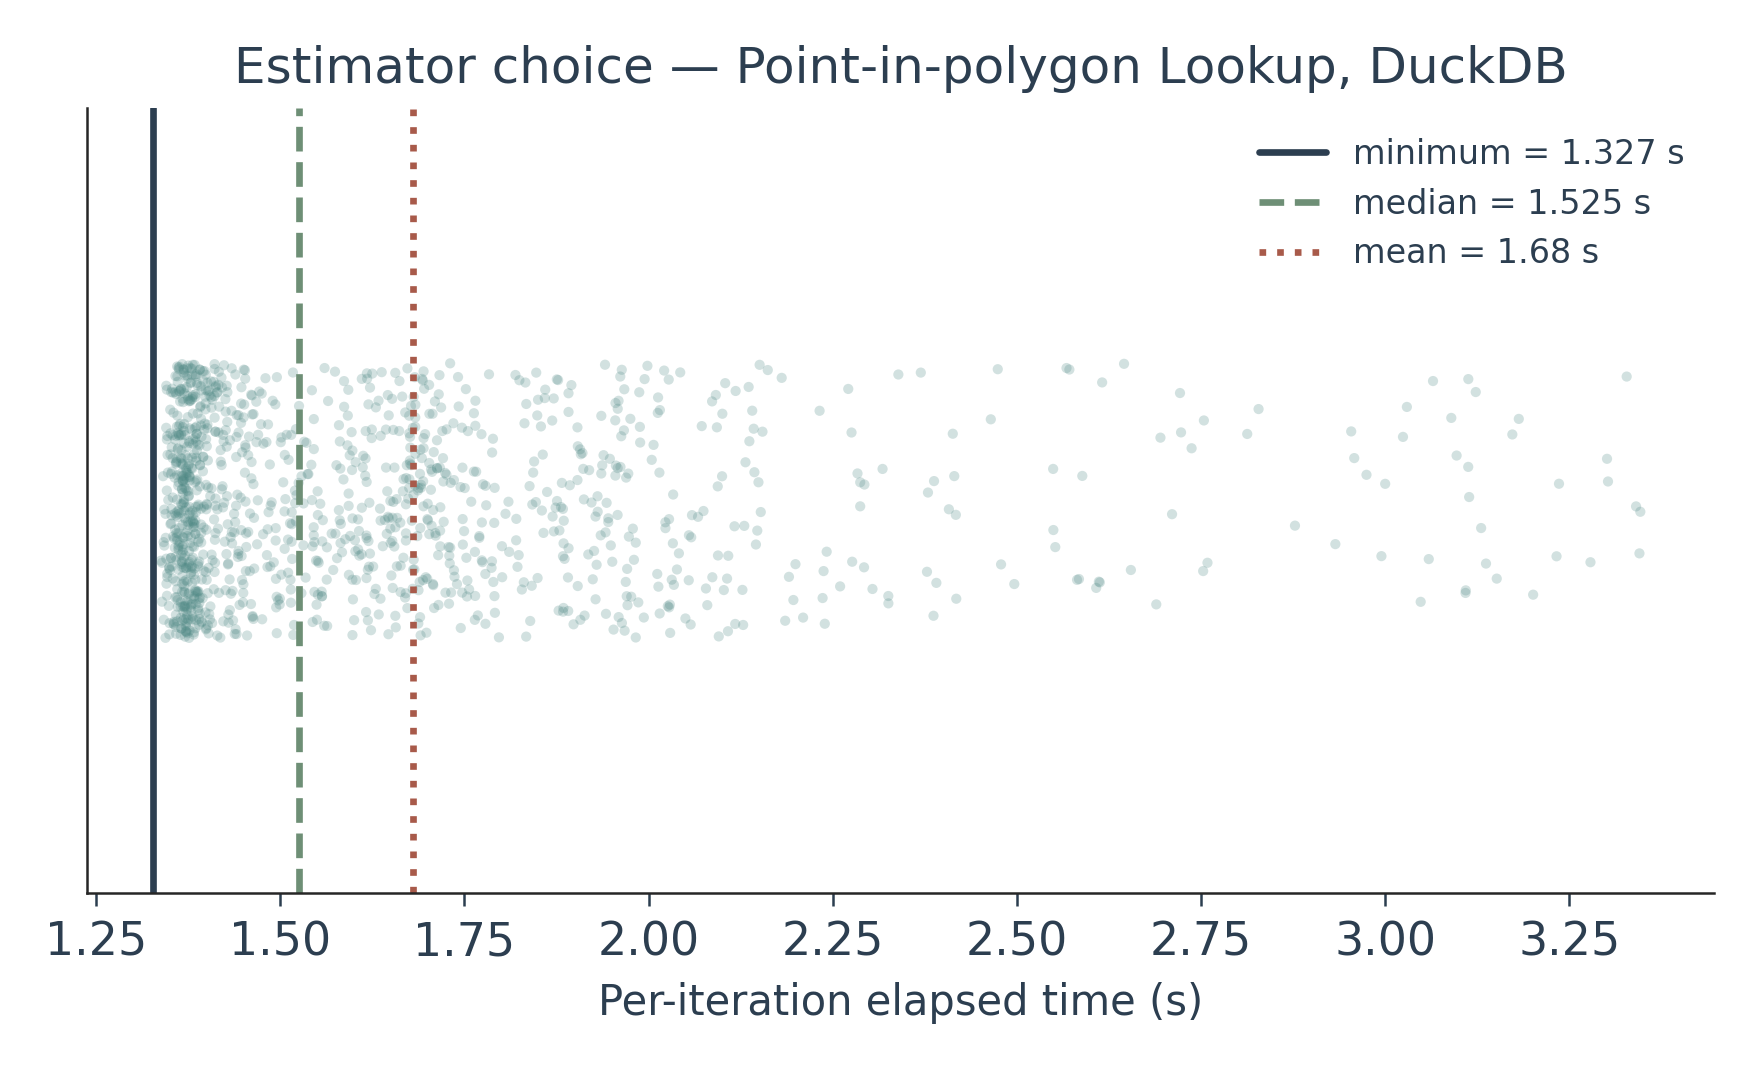
\includegraphics[width=0.7\textwidth]{Chapters/09-appendix/sub-chapters/figures/09-estimator-illustration.png}
    \caption[Minimum-versus-mean estimator illustration]{Per-iteration
    elapsed-time distribution for one representative query, with the minimum and
    the mean estimators marked. The separation between them is the one-sided
    contamination that motivates reporting the minimum
    \parencite{chen2016_robust_benchmarking_noisy_environments}.}
    \label{fig:appendix-estimator-illustration}
\end{figure}

\subsection{Run-to-run dispersion}
\label{appendix:supplementary-results:dispersion}

% TODO (prose): one sentence on the spread per configuration.

\begin{figure}[H]
    \centering
    % WHAT IT SHOWS: run-to-run dispersion -- the coefficient of variation (CV) of
    %   per-iteration elapsed time per configuration (optionally faceted by
    %   workload/tier).
    % CAPTION MUST STATE: that the y-axis is the CV; the per-configuration grouping;
    %   the workload/tier facet if used.
    % DESCRIPTIVE ONLY.
    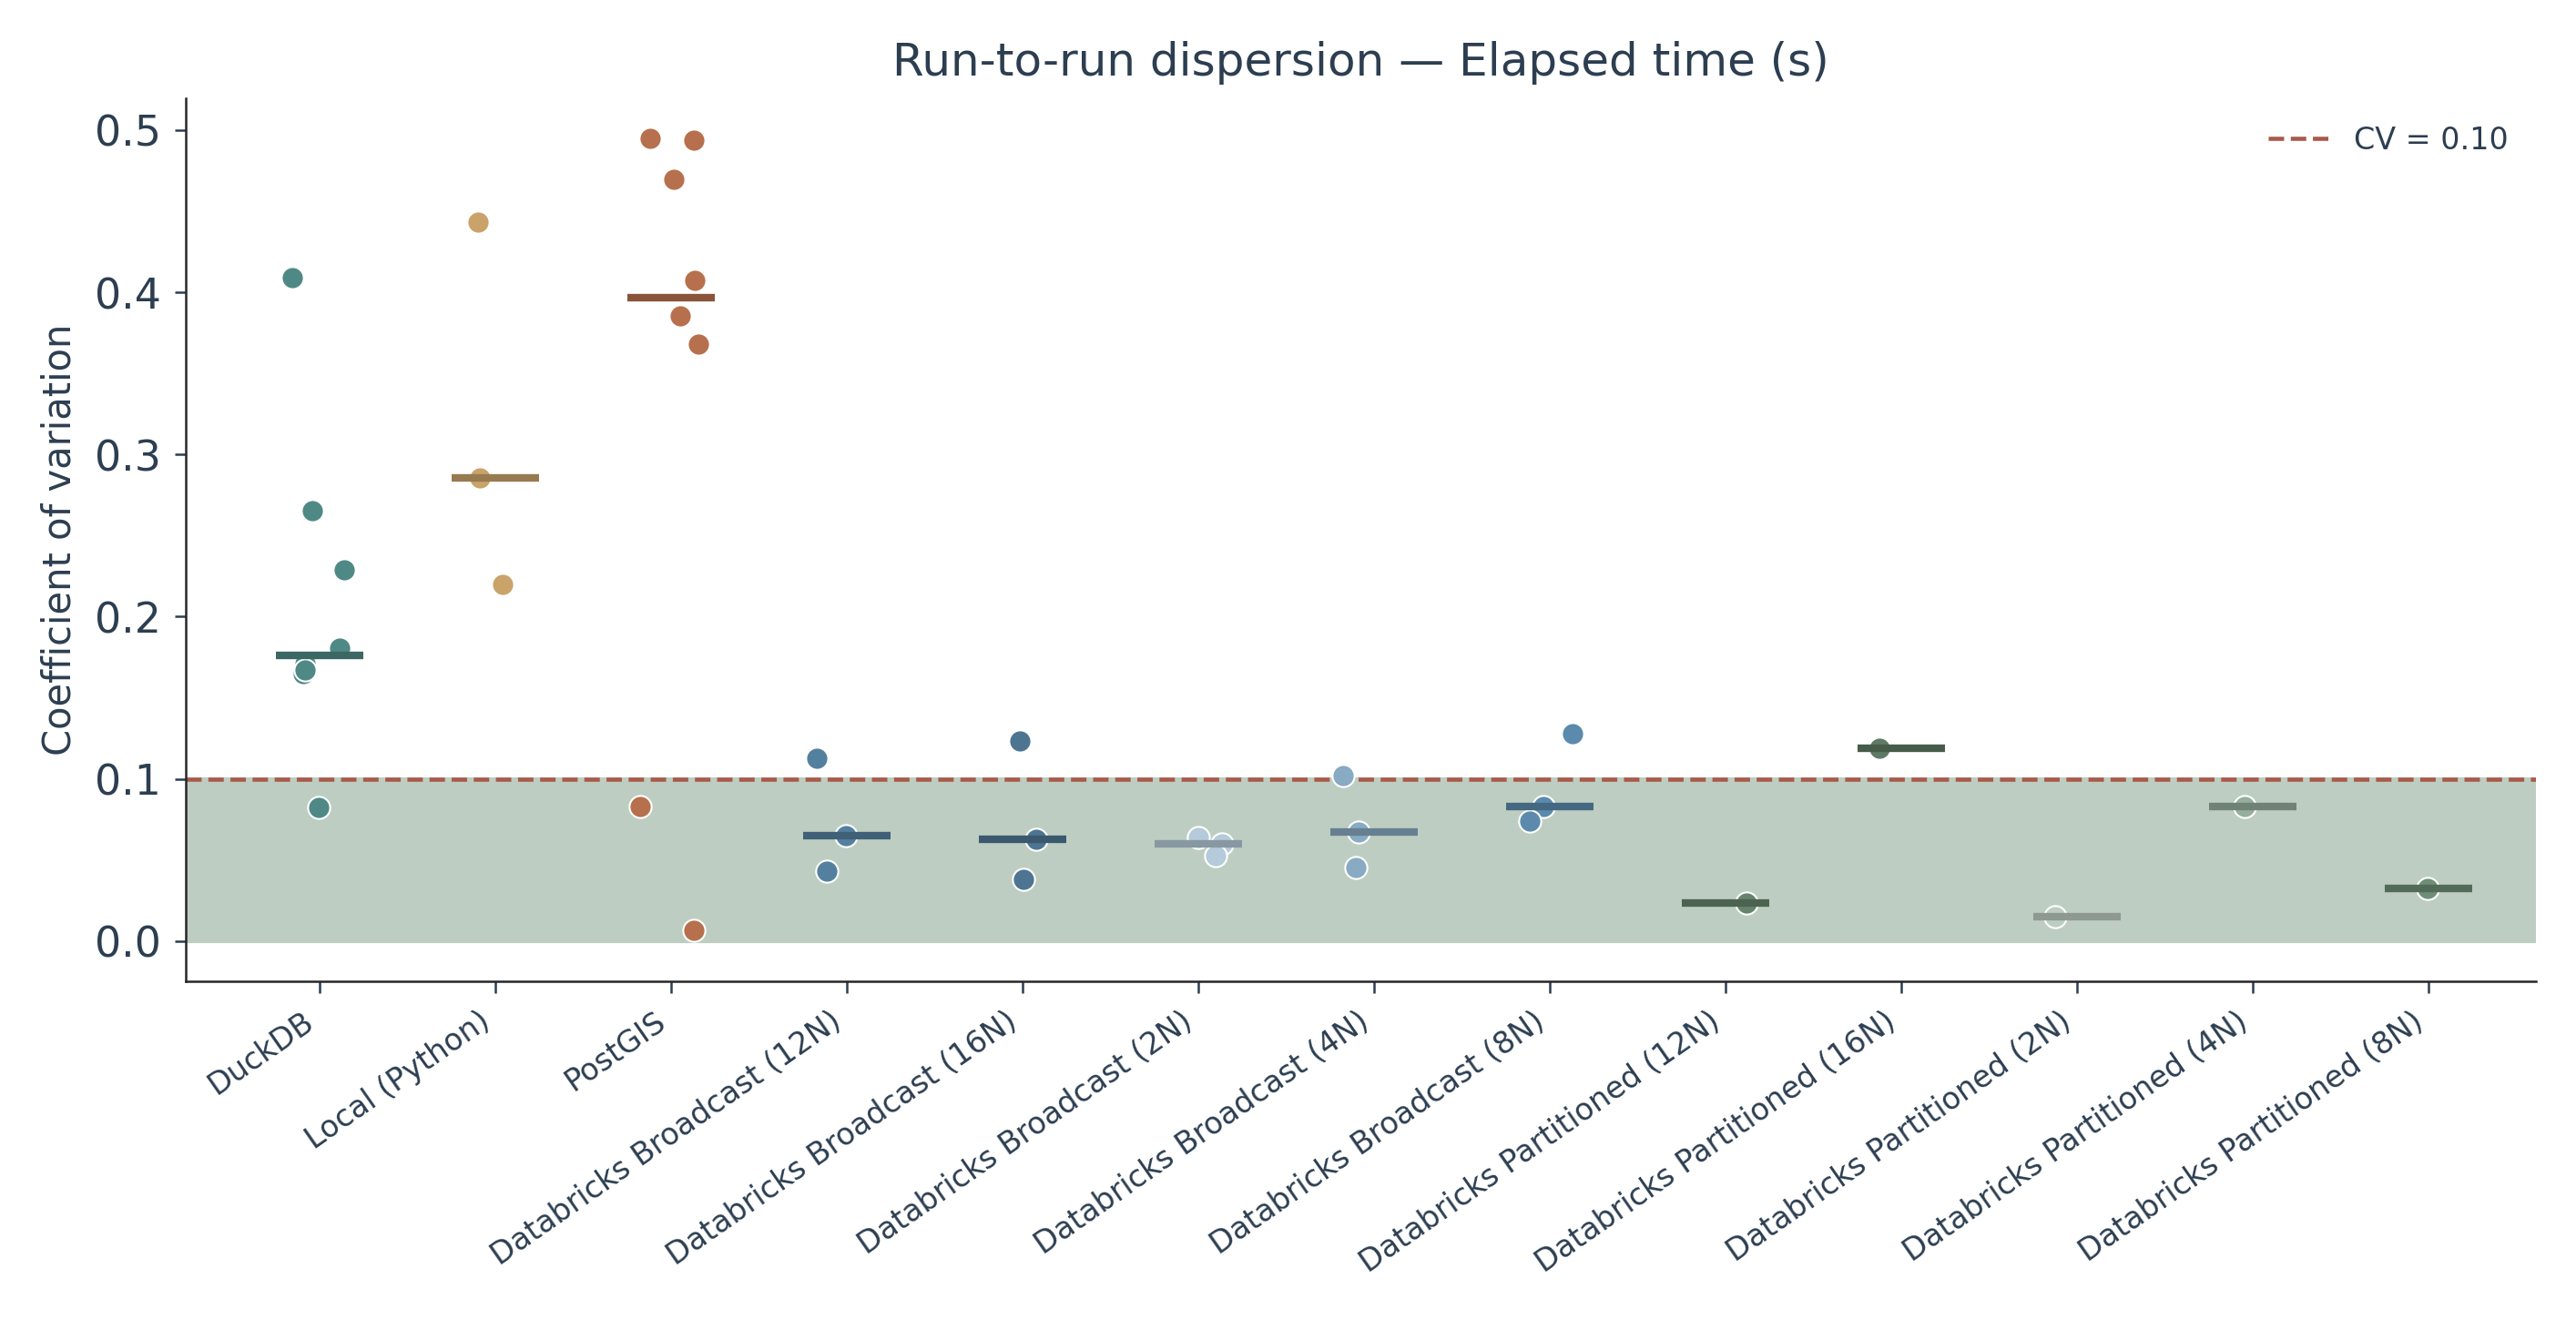
\includegraphics[width=0.75\textwidth]{Chapters/09-appendix/sub-chapters/figures/09-cv-dispersion.png}
    \caption[Run-to-run dispersion]{Run-to-run dispersion of per-iteration
    elapsed time, reported as the coefficient of variation per configuration. Bar
    colour encodes configuration using the thesis palette.}
    \label{fig:appendix-cv-dispersion}
\end{figure}

\subsection{CPU decomposition}
\label{appendix:supplementary-results:cpu-decomposition}

% TODO (prose): one sentence on the user-vs-system split.

\begin{figure}[H]
    \centering
    % WHAT IT SHOWS: CPU-time decomposition into user and system seconds per
    %   configuration (from psutil.Process.cpu_times), optionally per workload.
    % CAPTION MUST STATE: that bars split CPU time into user and system components;
    %   the per-configuration grouping; the source counter.
    % DESCRIPTIVE ONLY.
    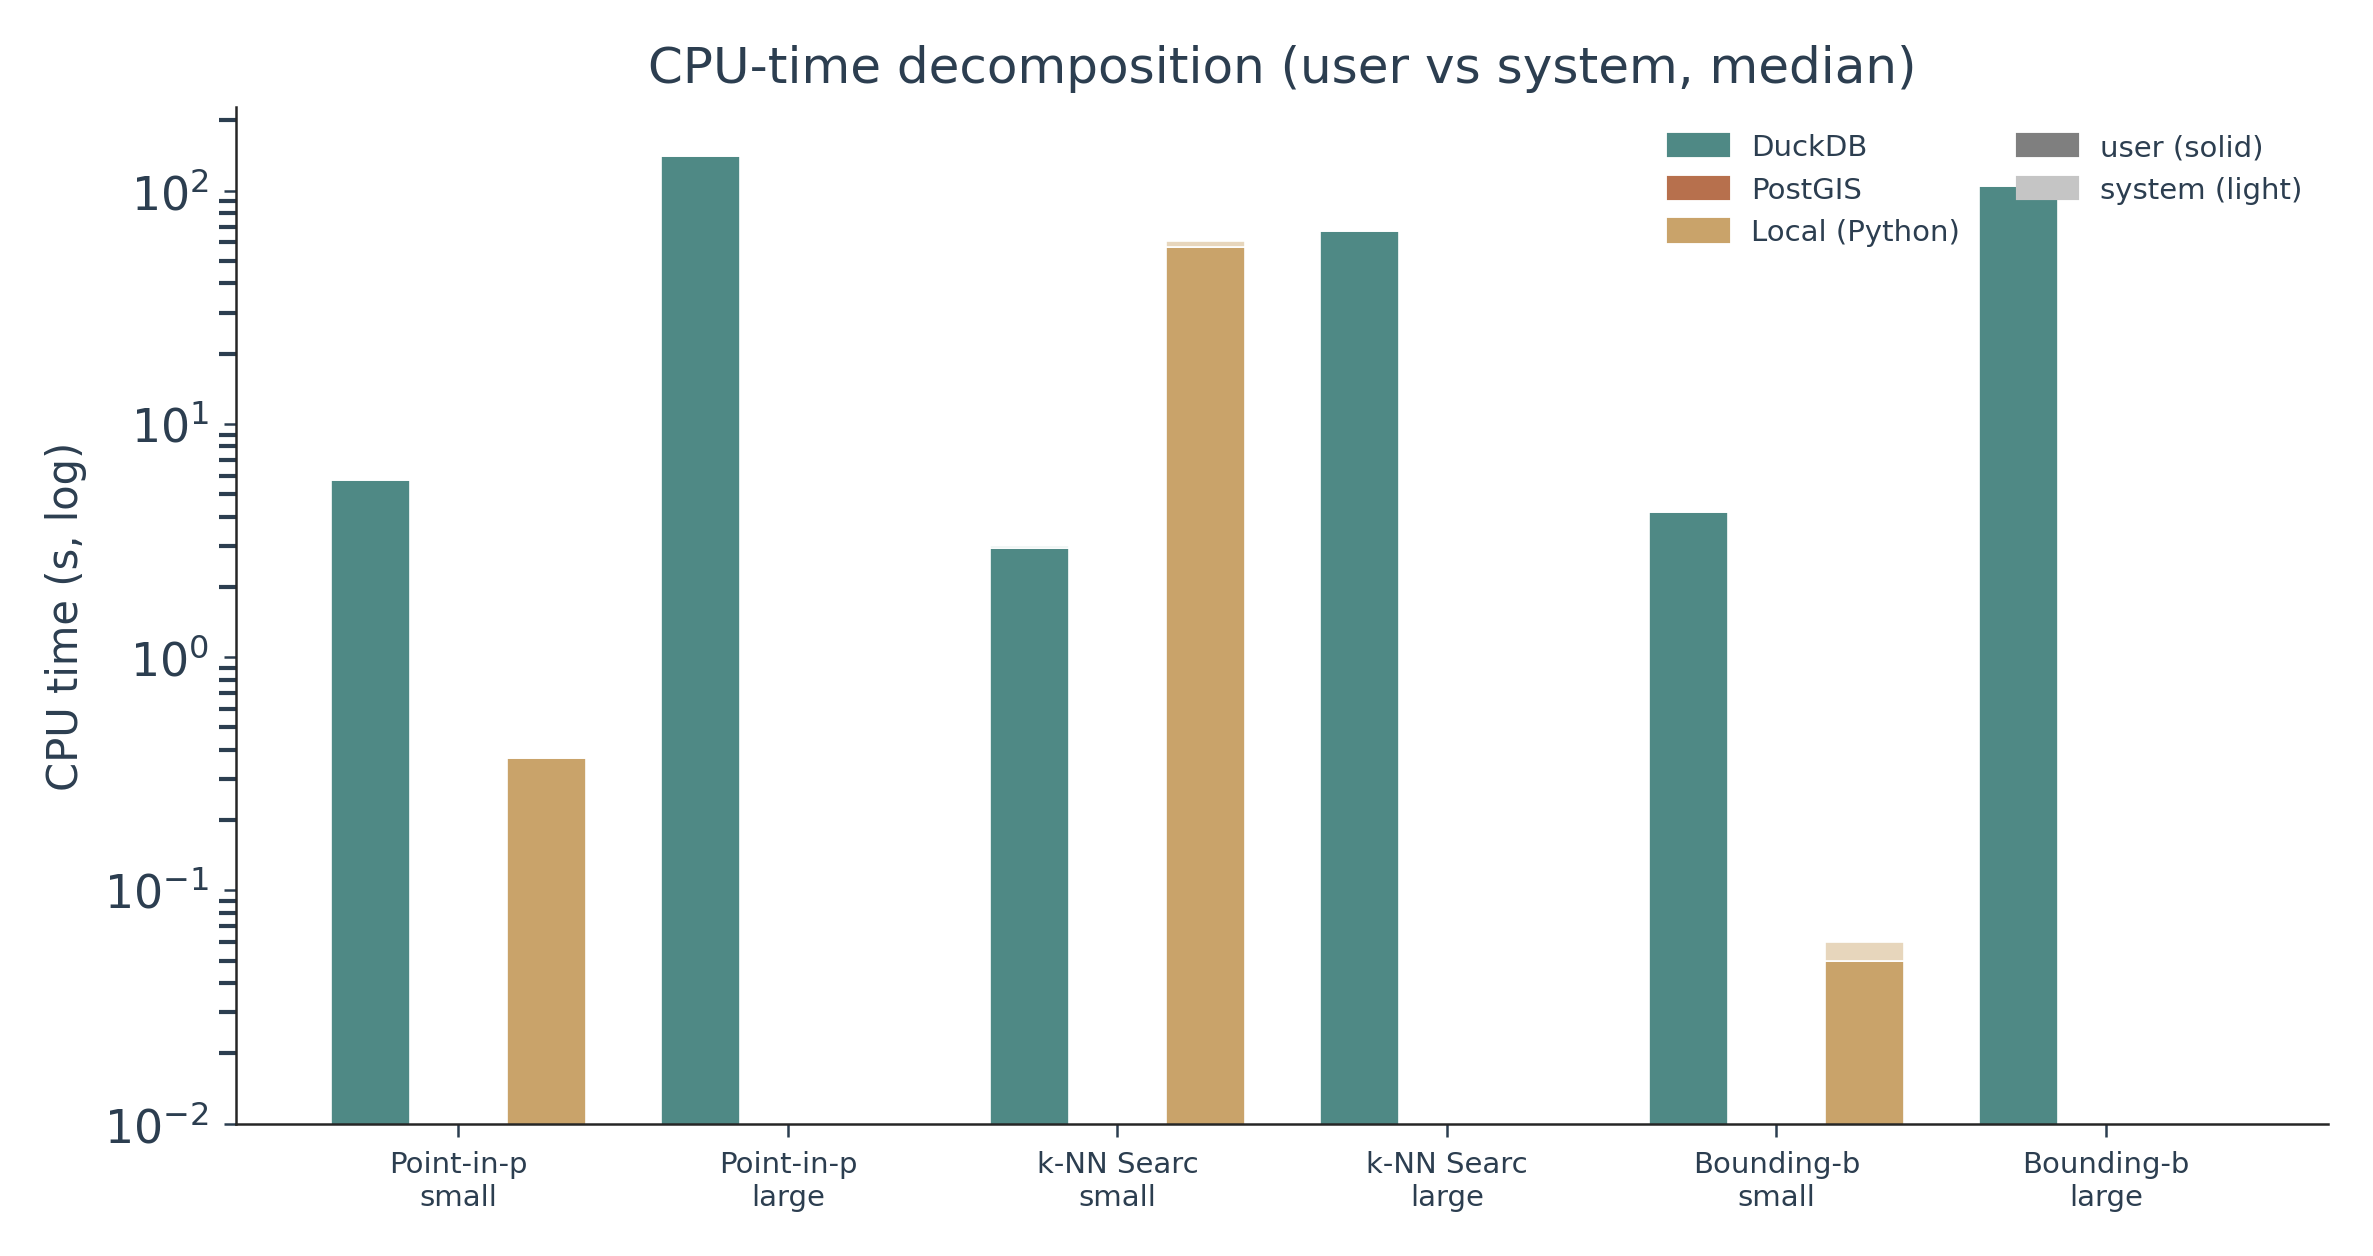
\includegraphics[width=0.75\textwidth]{Chapters/09-appendix/sub-chapters/figures/09-cpu-decomposition.png}
    \caption[CPU-time decomposition]{Process CPU time per configuration, split
    into user and system seconds. Component colour uses the thesis palette.}
    \label{fig:appendix-cpu-decomposition}
\end{figure}

\subsection{Per-cell chart grid}
\label{appendix:supplementary-results:cell-grid}

% TODO (prose): one sentence -- this auto-generated grid is the completeness view
% behind the chapter figures.

\begin{figure}[H]
    \centering
    % WHAT IT SHOWS: the auto-generated per-cell chart grid -- one panel per
    %   (workload x tier) cell, each panel carrying the median bars, the violin of
    %   the per-iteration distribution, network I/O, and cost.
    % CAPTION MUST STATE: that this is the auto-generated completeness grid; the
    %   per-cell panel contents; that it absorbs within-configuration size-scaling
    %   and the cross-workload median bars.
    % NOTE: this is the auto-generated completeness grid; it is large and may span
    %   a full page (consider a dedicated landscape page when the artwork exists).
    % DESCRIPTIVE ONLY.
    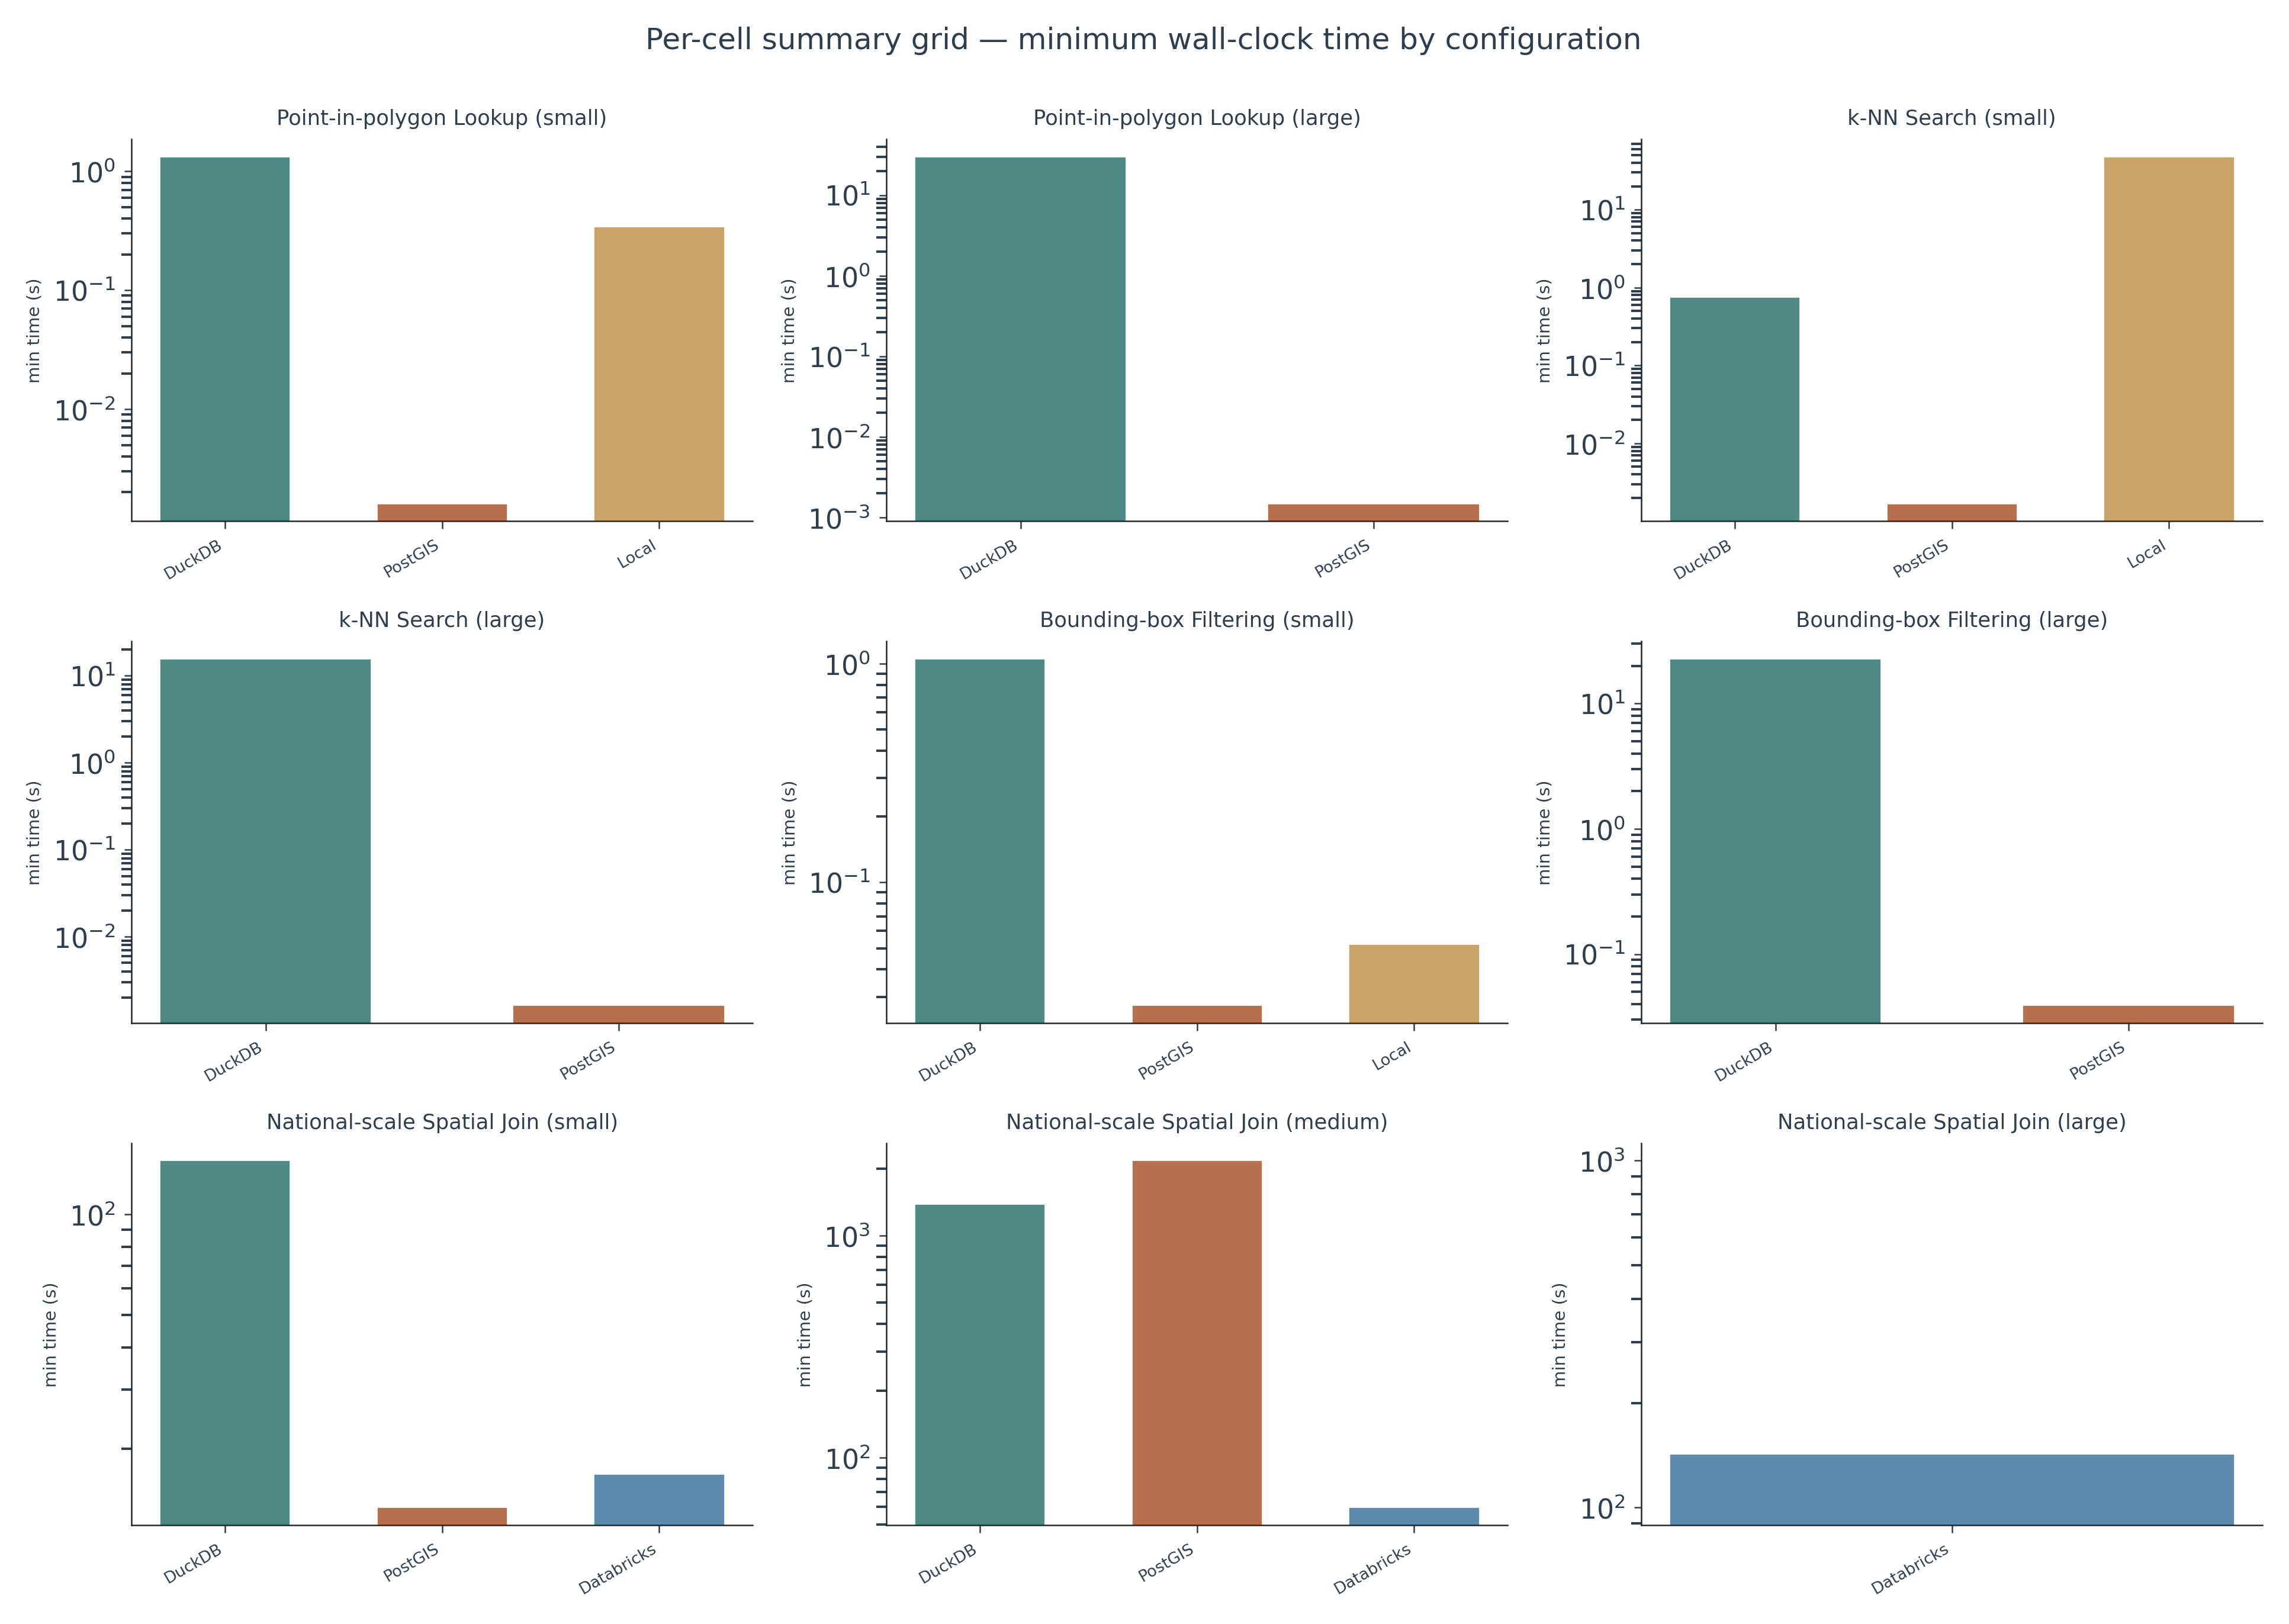
\includegraphics[width=\textwidth]{Chapters/09-appendix/sub-chapters/figures/09-cell-grid.png}
    \caption[Per-cell chart grid]{Auto-generated per-cell chart grid, one panel per
    workload pattern and size tier, each carrying the median bars, the per-iteration
    distribution violin, the network I/O, and the cost. The grid is the
    completeness view that absorbs within-configuration size-scaling and the
    cross-workload median bars.}
    \label{fig:appendix-cell-grid}
\end{figure}

\subsection{Storage footprint}
\label{appendix:supplementary-results:storage-footprint}

% TODO (prose): one sentence on each format's on-disk footprint vs. input size.

\begin{table}[H]
    \centering
    % WHAT IT SHOWS: storage footprint per format (GeoParquet, PostGIS table,
    %   Shapefile) against the input dataset size, per size tier.
    % CAPTION MUST STATE: the formats compared; that footprint is on-disk bytes;
    %   the per-tier breakdown.
    % DATA: leave data rows commented out -- do NOT invent numbers.
    \footnotesize
    \setlength{\tabcolsep}{8pt}
    \renewcommand{\arraystretch}{1.2}
    \begin{tabular}{@{}l r r r r@{}}
        \toprule
        \textbf{Tier} & \textbf{Input} & \textbf{GeoParquet} & \textbf{PostGIS} & \textbf{Shapefile} \\
        \midrule
        % TODO: one row per tier; values are on-disk sizes. No real numbers:
        % Small  & <size> & <size> & <size> & <size> \\
        % ...
        \bottomrule
    \end{tabular}
    \caption[Storage footprint per format]{On-disk storage footprint of each format
    against the input dataset size, per size tier.}
    \label{tab:appendix-storage-footprint}
\end{table}

\subsection{Raw Spark-internal metrics}
\label{appendix:supplementary-results:spark-metrics}

% TODO (prose): one sentence pointing to the raw distributions behind the RQ2
% phase breakdown (Figure~\ref{fig:distributed-execution-phase-breakdown}).

\begin{figure}[H]
    \centering
    % WHAT IT SHOWS: distributions of the raw Databricks Spark-internal metrics
    %   captured by the SparkListener -- executorRunTime, inputMetrics.bytesRead,
    %   shuffle read/write bytes, and per-stage durations -- across iterations and
    %   worker counts.
    % CAPTION MUST STATE: which Spark-internal metrics are shown; that these are
    %   the raw per-stage distributions feeding the phase breakdown; the axes.
    % DESCRIPTIVE ONLY.
    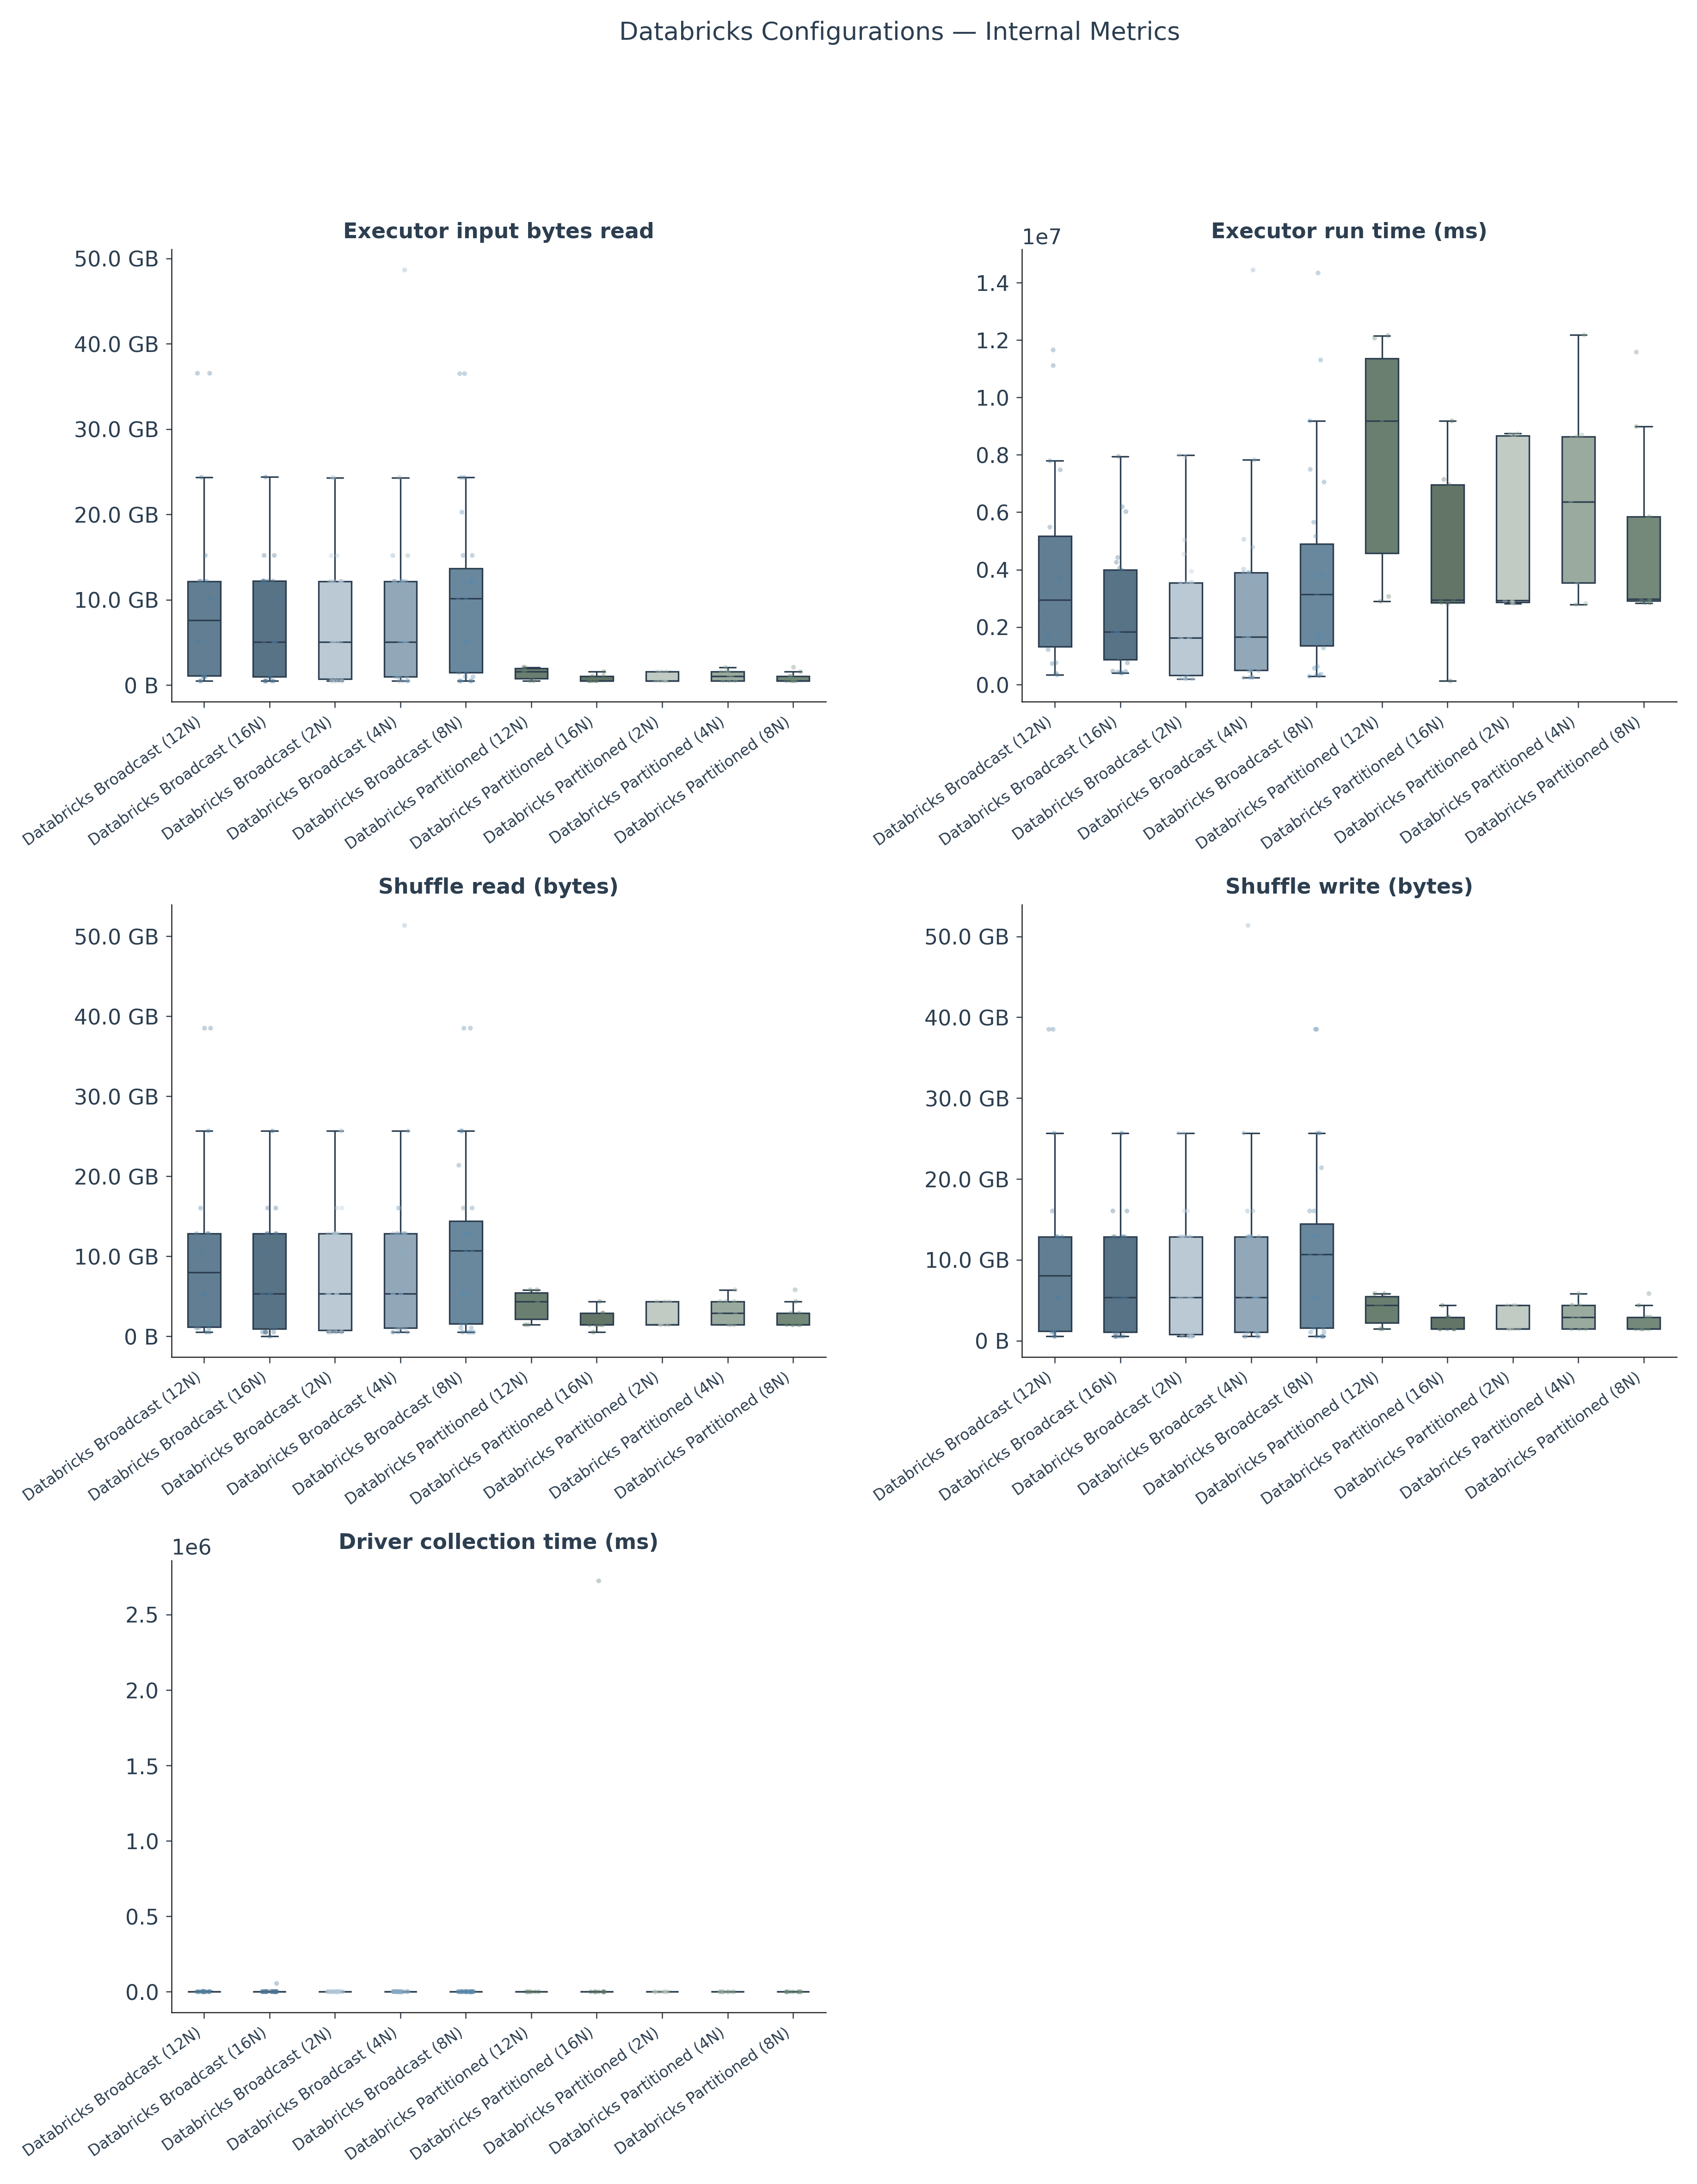
\includegraphics[width=0.9\textwidth]{Chapters/09-appendix/sub-chapters/figures/09-spark-metrics.png}
    \caption[Raw Spark-internal metric distributions]{Distributions of the raw
    Databricks Spark-internal metrics recorded by the \texttt{SparkListener} --
    executor run time, input bytes read, shuffle bytes read and written, and
    per-stage durations -- across iterations and worker counts. These are the raw
    quantities that feed the execution-phase breakdown of
    Figure~\ref{fig:distributed-execution-phase-breakdown}.}
    \label{fig:appendix-spark-metrics}
\end{figure}
